\documentclass[tikz,border=3pt]{standalone}
\usepackage{amsmath,amssymb}
\usepackage{sourcesanspro}
\usetikzlibrary{arrows.meta, positioning, calc}

\definecolor{cPrimal}{RGB}{0, 102, 180}
\definecolor{cDual}{RGB}{209, 34, 57}
\definecolor{govGreen}{RGB}{16, 128, 64}

\begin{document}
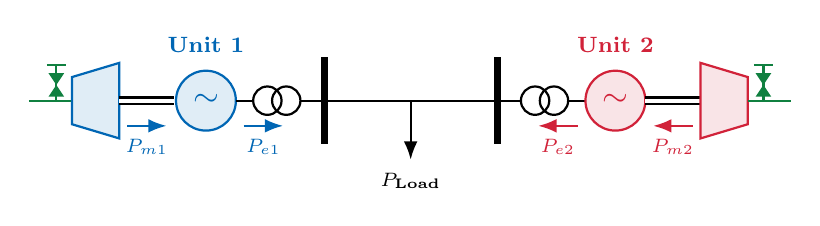
\begin{tikzpicture}[>=Latex, font=\footnotesize]

    % ========================================================
    % UNIT 1 (LEFT) - Blue theme
    % ========================================================
    \node[above=2pt, font=\bfseries\footnotesize, cPrimal] at (1.9, 0.42) {Unit 1};
    
    % Steam pipe & Valve 1
    \draw[thick, govGreen] (-0.35, 0) -- (0.0, 0);
    \draw[thick, govGreen] (0.0, 0.0) -- (0.0, 0.45);
    \draw[thick, govGreen] (-0.12, 0.45) -- (0.12, 0.45);
    \fill[govGreen] (-0.1, 0.35) -- (0.1, 0.35) -- (0, 0.2) -- cycle;
    \fill[govGreen] (-0.1, 0.05) -- (0.1, 0.05) -- (0, 0.2) -- cycle;
    \draw[thick, govGreen] (0.0, 0.0) -- (0.2, 0.0);
    
    % Turbine 1 (trapezoid expanding to the right)
    \draw[thick, fill=cPrimal!12, draw=cPrimal] (0.2, -0.3) -- (0.8, -0.48) -- (0.8, 0.48) -- (0.2, 0.3) -- cycle;
    
    % Shaft 1
    \draw[thick, double, double distance=1.5pt] (0.8, 0) -- (1.5, 0);
    
    % Generator 1
    \draw[thick, fill=cPrimal!12, draw=cPrimal] (1.9, 0) circle (0.38);
    \node[cPrimal, font=\large] at (1.9, 0) {$\sim$};
    
    % Transformer 1
    \draw[thick] (2.28, 0) -- (2.5, 0);
    \draw[thick] (2.68, 0) circle (0.18);
    \draw[thick] (2.92, 0) circle (0.18);
    \draw[thick] (3.1, 0) -- (3.4, 0);
    
    % Busbar 1
    \draw[ultra thick, line width=2.5pt] (3.4, -0.55) -- (3.4, 0.55);
    
    % Power arrows Unit 1
    \draw[->, thick, cPrimal] (0.9, -0.32) -- (1.4, -0.32) node[midway, below=1pt, font=\scriptsize] {$P_{m1}$};
    \draw[->, thick, cPrimal] (2.38, -0.32) -- (2.88, -0.32) node[midway, below=1pt, font=\scriptsize] {$P_{e1}$};

    % ========================================================
    % INTERCONNECTION & LOAD (CENTER)
    % ========================================================
    \draw[thick] (3.4, 0) -- (5.6, 0);
    \draw[thick] (4.5, 0) -- (4.5, -0.35);
    \draw[->, thick] (4.5, -0.35) -- (4.5, -0.75) node[below=1pt, font=\bfseries\scriptsize] {$P_{\text{Load}}$};

    % ========================================================
    % UNIT 2 (RIGHT) - Red theme
    % ========================================================
    \node[above=2pt, font=\bfseries\footnotesize, cDual] at (7.1, 0.42) {Unit 2};
    
    % Busbar 2
    \draw[ultra thick, line width=2.5pt] (5.6, -0.55) -- (5.6, 0.55);
    
    % Transformer 2
    \draw[thick] (5.6, 0) -- (5.9, 0);
    \draw[thick] (6.08, 0) circle (0.18);
    \draw[thick] (6.32, 0) circle (0.18);
    \draw[thick] (6.5, 0) -- (6.72, 0);
    
    % Generator 2
    \draw[thick, fill=cDual!12, draw=cDual] (7.1, 0) circle (0.38);
    \node[cDual, font=\large] at (7.1, 0) {$\sim$};
    
    % Shaft 2
    \draw[thick, double, double distance=1.5pt] (7.48, 0) -- (8.18, 0);
    
    % Turbine 2 (trapezoid expanding to the left towards shaft)
    \draw[thick, fill=cDual!12, draw=cDual] (8.18, -0.48) -- (8.78, -0.3) -- (8.78, 0.3) -- (8.18, 0.48) -- cycle;
    
    % Steam pipe & Valve 2
    \draw[thick, govGreen] (8.78, 0.0) -- (8.98, 0.0);
    \draw[thick, govGreen] (8.98, 0.0) -- (8.98, 0.45);
    \draw[thick, govGreen] (8.86, 0.45) -- (9.10, 0.45);
    \fill[govGreen] (8.88, 0.35) -- (9.08, 0.35) -- (8.98, 0.2) -- cycle;
    \fill[govGreen] (8.88, 0.05) -- (9.08, 0.05) -- (8.98, 0.2) -- cycle;
    \draw[thick, govGreen] (8.98, 0) -- (9.33, 0);
    
    % Power arrows Unit 2 (flowing leftwards into the grid)
    \draw[->, thick, cDual] (8.08, -0.32) -- (7.58, -0.32) node[midway, below=1pt, font=\scriptsize] {$P_{m2}$};
    \draw[->, thick, cDual] (6.62, -0.32) -- (6.12, -0.32) node[midway, below=1pt, font=\scriptsize] {$P_{e2}$};

\end{tikzpicture}
\end{document}
